%%%%%%%%%%%%%%%%%%%%%%%%%%%%%%%%%%%%%%%%%%%%%%%%%%%%%%%%%%%%%%%%%%%%%%%%%%%%%%%%
\chapter{Анализ существующих решений}
%%%%%%%%%%%%%%%%%%%%%%%%%%%%%%%%%%%%%%%%%%%%%%%%%%%%%%%%%%%%%%%%%%%%%%%%%%%%%%%%

\section{Информационные системы}

Информационные системы - это взаимосвязанная совокупность средств, методов и персонала, используемых для хранения, обработки и выдачи информации для достижения цели управления. 

\subsection{Способы аналитики информационных систем}

В информационных системах доступны следующие способы анализа и визуального представления результатов:

\begin{enumerate}
	\item Инструменты для анализа данных. Это специальные программы, дающие возможность создания отчётов, диаграмм и срезов данных. Особенностью таких отчётов является простота использования за счёт графического интерфейса. Такие отчёты могут выполнять непосредственно работники, использующие систему.
	
	\item Программные отчёты. Такие отчёты используются в случаях, когда функциональности мастеров отчётов недостаточно. Программные отчёты требуют более широкого знания системы и навыков написания на языке SQL. Обычно такой способ - это трудоёмкий ручной процесс, требующий специальных навыков. 
\end{enumerate}

\subsection{Инструменты аналитики Vtiger}

CRM система – это программное обеспечение, предназначенное для сбора и хранения всей информации, связанной с клиентами, а также автоматизации взаимодействий с ними. Целю CRM является предоставление полного набора данных о клиентах, который может использоваться для увеличения продаж, удержания, привлечения и повышения уровня обслуживания клиентов.

Vtiger CRM - это система управления взаимоотношениями с клиентами с открытым кодом и возможностью создания пользовательских модулей. Vtiger CRM предоставляет сделующие средства для анализа и интеллектуальной обработки данных: отчёты, контрольные панели и виджеты. 

"\textbf{Виджет} - это небольшой графический элемент, выводимый на главную страницу системы Vtiger CRM, либо на страницу “Виджеты” для любых Модулей системы." \cite{salesplatform}
	
Виджет, как можно увидеть на рисунке \ref{fig:widget}, визуализирует представление данных в системе. На одном экране можно поместить сразу несколько виджетов.
	
\begin{figure}[htbp]
	\centering
	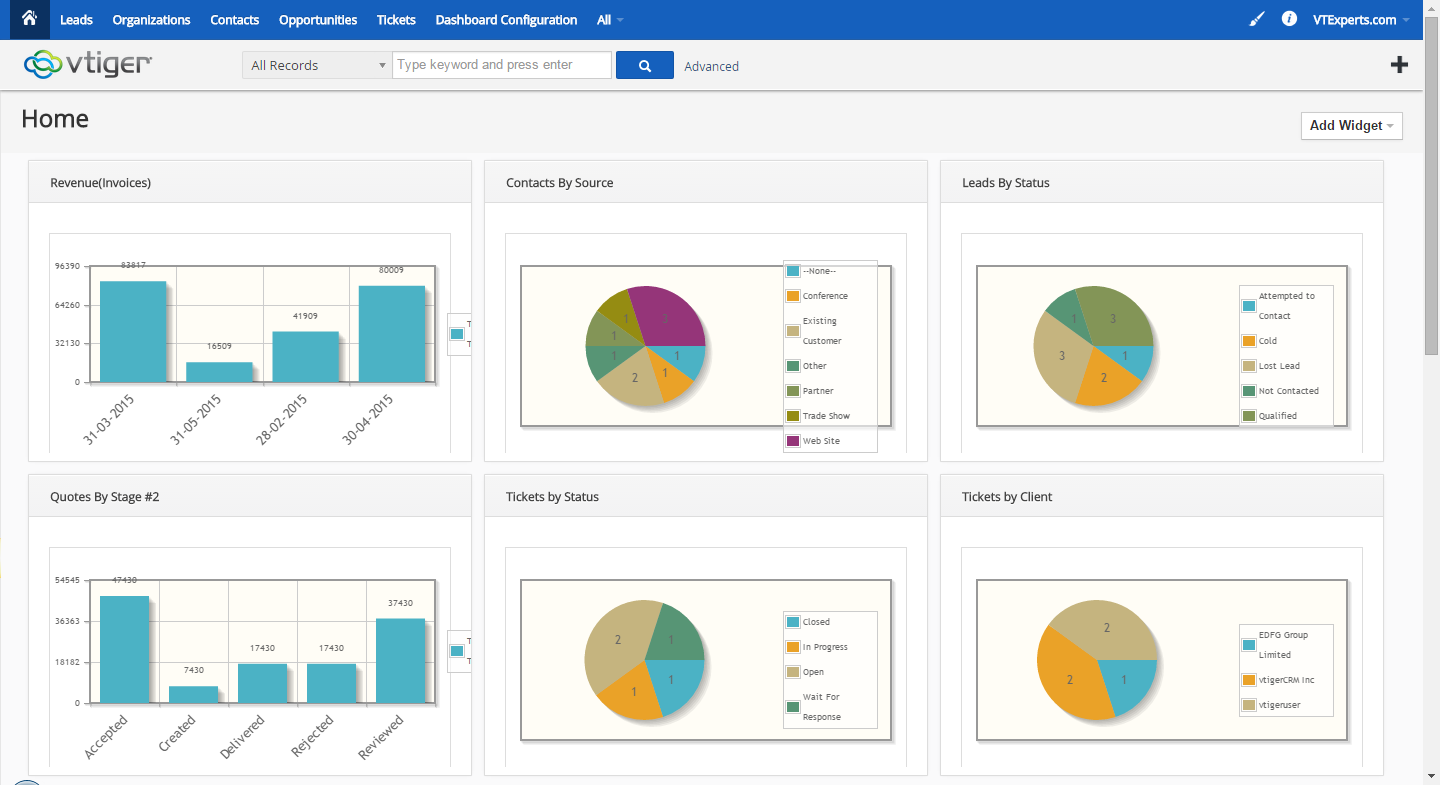
\includegraphics[width=0.9\textwidth]{fig/chapter_1/widget}
	\caption{Пример виджетов Vtiger}
	\label{fig:widget}
\end{figure}

Другим средством является \textbf{Модуль Отчёты}, который собирает, фильтрует и организовывает данные в виде таблиц и диаграмм. Системой Vtiger CRM предоставляется генератор и дизайнер отчётов:

\begin{itemize}
	\item Генератор отчетов создает отчеты, которые можно просматривать и выводить в файлы PDF или Excel.
	
	\item Дизайнер отчетов даёт возможность выбирать данные, которые необходимо включить в отчет, и создать представление данных в отчете.
\end{itemize}

Как видно на рисунке \ref{fig:rep_1}, Vtiger предлагает множество вариантов составления стандартных отчётов.

\begin{figure}[htbp]
	\centering
	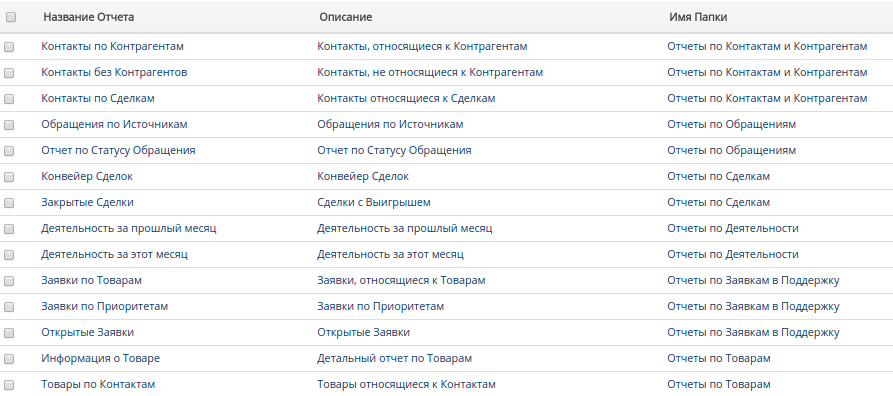
\includegraphics[width=1\textwidth]{fig/chapter_1/rep_1}
	\caption{Список стандартных отчётов}
	\label{fig:rep_1}
\end{figure}

Существует два вида отчётов: \textbf{диаграммы и детальные отчёты}. Детальные отчёты дают возможность пользователю получить релевантные для него данные в табличной форме. Пример такого отчёта на рисунке \ref{fig:rep_2}.

Диаграмма в свою очередь - это визуальное представление данных в виде круговой или столбиковой диаграммы, или линейного графика. Пример диаграммы на рисунке \ref{fig:diag}.

\begin{figure}[htbp]
	\centering
	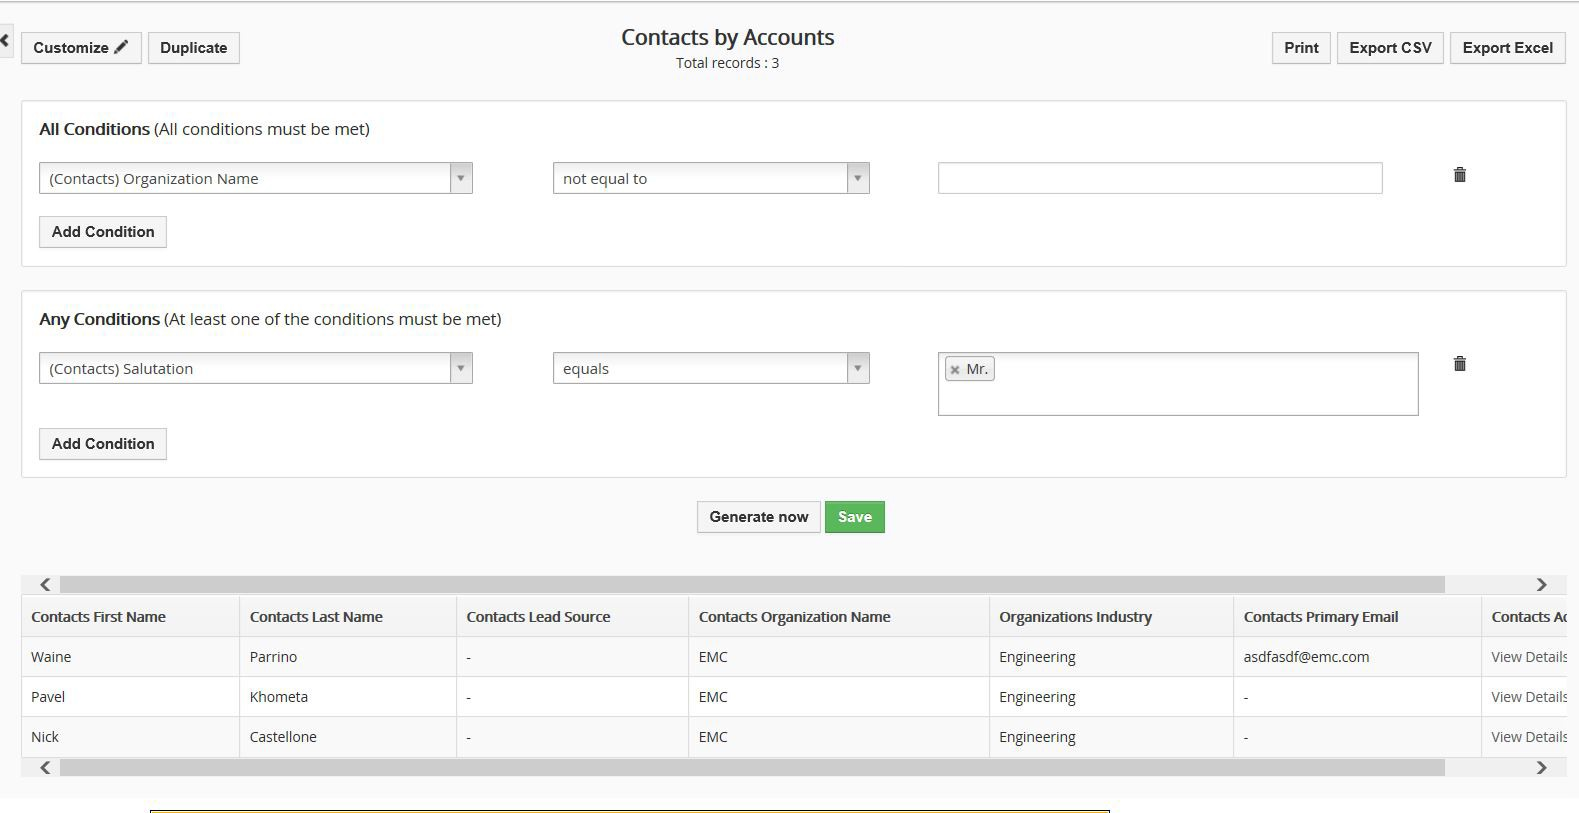
\includegraphics[width=1\textwidth]{fig/chapter_1/rep_2}
	\caption{Пример детального отчёта}
	\label{fig:rep_2}
\end{figure}

\begin{figure}[htbp]
	\centering
	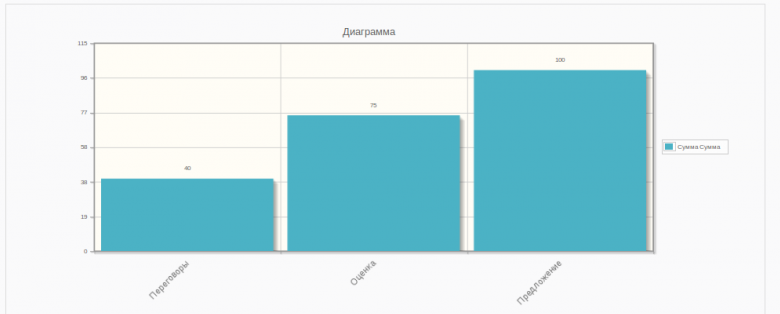
\includegraphics[width=.65\textwidth]{fig/chapter_1/diag}
	\caption{Пример отчёта-диаграммы}
	\label{fig:diag}
\end{figure}
\newpage

Обоим видам отчётов необходима дополнительная настройка с использованим фильтров. Однако они не всегда являются полными для аналитики, так как относятся только к сфере продаж и маркетинга. Также, в таких отчётах отсутствует гибкость.

\nocite{vtiger}

\section{Системы бизнес-аналитики}

Business Intellegence (BI) системы - это аналитические системы, которые объединяют данные из различных источников информации, обрабатывают их и предоставляют удобный интерфейс для изучения и оценки полученных сведений.\cite{bi} Структура BI платформы представлена на рисунке \ref{fig:bi}.

\begin{figure}[htbp]
	\centering
	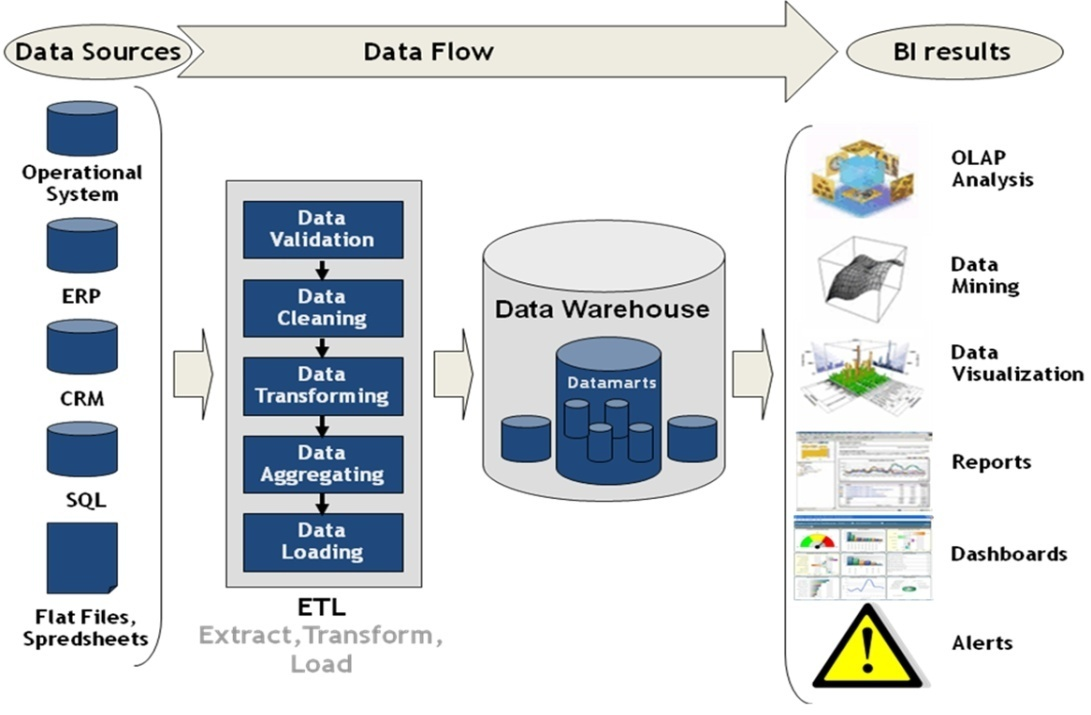
\includegraphics[width=.75\textwidth]{fig/chapter_1/bi}
	\caption{Структура BI платформы}
	\label{fig:bi}
\end{figure}

\subsection{Анализ данных платформы Pentaho BI}

Pentaho BI - свободно распространяющаяся система бизнес-аналитики. Сервер платформы написан на языке Java и предоставляет инфраструктуру для отображения отчётов через веб-сервисы. 

В платформе Pentaho есть два основных варианта анализа данных: Pentaho Reporting и Mondrian OLAP Server.

\begin{enumerate}
	\item Pentaho Reporting - это набор инструментов для создания детальных отчётов. \cite{report} 
	
	С помощью Pentaho Reporting можно преобразовывать данные в  приспособленную для клиентов значимую информацию. В Pentaho Reporting возможно создавать отчеты в форматах HTML, Excel, PDF, Text, XML, CSV, или печатной форме. 
	
	Также одним из преимуществ является отсутствие требований к знаниям о системе и простота в использовании (рисунок \ref{fig:pentaho_rep}).
	
	\begin{figure}[htbp]
		\centering
		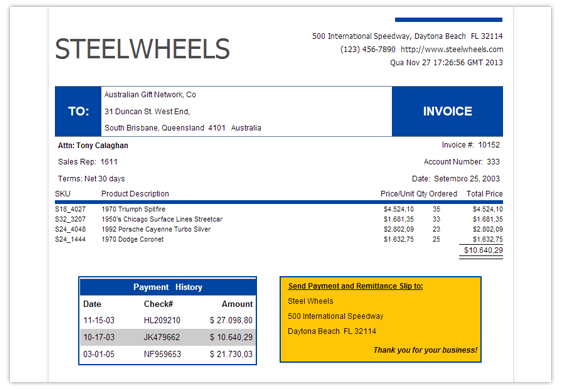
\includegraphics[width=.9\textwidth]{fig/chapter_1/pentaho_rep}
		\caption{Отчёт в Pentaho Reporting}
		\label{fig:pentaho_rep}
	\end{figure}

	\item Mondrian OLAP Server позволяет пользователям анализировать сразу большие массивы данных, строить прогнозы и сценарии, а также разрабатывать множество вариантов планов за счёт OLAP-технологии многомерных кубов. При построении аналитического отчёта пользователь делает срезы измерений гиперкуба, чтобы изолировать и найти необходимые данные. Это даёт гибкость предоставления анализируемых данных. Также пользователю не обязательно знать языки выборки, и необходимы минимальные знания системы. Пример аналитического отчёта приведён на рисунке \ref{fig:saiku}. 
	
	\begin{figure}[htbp]
		\centering
		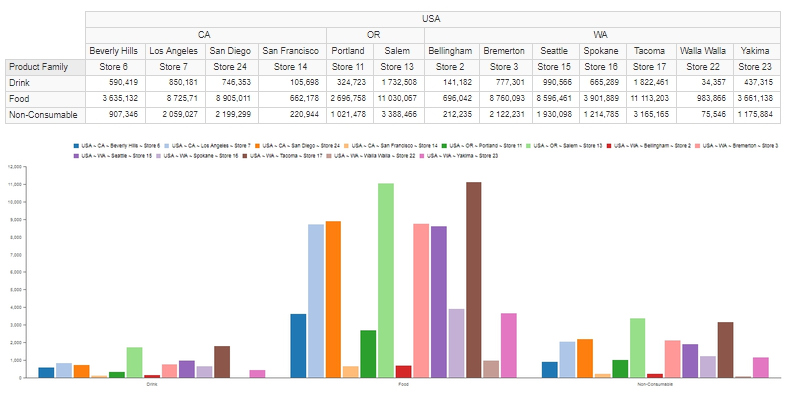
\includegraphics[width=.9\textwidth]{fig/chapter_1/saiku}
		\caption{Отчёт, построенный инструментом Saiku}
		\label{fig:saiku}
	\end{figure}
\end{enumerate}

Сравнение представлено в таблице \ref{tab:rep_an}:

\tabulinesep = 1mm
\begin{longtabu} to \textwidth {| X[c,m] | X[c,m] |}
	\firsthline\hline
	Reporting & Analysis\\ \hline
	\endfirsthead
	Преобразует данные в информацию & Преобразует данные и информацию в ответы\\ \hline
	Вызывает вопросы о бизнесе у своих конечных пользователей & Отвечает на вопросы, интерпретируя данные на более глубоком уровне и предоставляя действенные рекомендации\\ \hline
	Показывает, что произошло & Показывает, почему это произошло и что с этим можно сделать\\ \hline
	\caption{Сравнение Reporting и Analysis}
	\label{tab:rep_an}
\end{longtabu}

За отчётностью идёт аналитика, чтобы ответить на появившиеся вопросы.

\subsubsection{Конструкторы аналитических отчётов}

Pentaho BI обладает несколькими приложениями для построения аналитических отчётов:

\begin{enumerate}
	\item \textbf{Jpivot} - это библиотека пользовательских тегов JSP, которая отображает таблицу OLAP и позволяет пользователям выполнять типичные OLAP-навигации. Поддержка данного инструмента разработчиками завершилась в 2008 году, из-за чего он, на данный момент, является наименее удобным и бытрым вариантом построения аналитических отчётов.
	
	\item \textbf{Saiku} является приложением OLAP-анализа. Обладает легковесной архитектурой клиента, а также простой реализацией REST-API. Скорость работы данного инструмента выше, чем у остальных представленных конструкторов аналитических отчётов.
	
	\item \textbf{Pivot4j} - Java API для OLAP-серверов. Предоставляет широкие возможности для реализации независимого API. Pivot4j практически все операции выполняет на стороне сервера. Однако, реализация REST-приложения сложнее, чем у Saiku.
\end{enumerate}

\section{Интеграция BI и информационной системы}

Хотя, и BI и CRM решения относятся к сбору и анализу данных, однако, если BI, предоставляет пользователю принимать решения, то CRM, напротив, позволяет пользователям участвовать в любом процессе анализа данных и автоматизирует их.

Очевидно, что связь приложения CRM с системой бизнес-аналитики даёт преимущества обеих систем(эффективный анализ со стороны BI и улучшение и автоматизация взаимодействия с клиентами и увеличение клиентской базы). BI обрабатывает большие объёмы информации, а CRM-система выступает провайдером данных. Однако, такая связь обычно приводит также к дополнительным затратам на приобритение программных средств.

Кроме того, для добавления пользовательских модулей и построения нестандартных отчётов в CRM-системе необходимо изучить язык программирования, на котором написано CRM-приложение. Использование бизнес-аналитики позволит сократить необходимость дополнительных знаний в CRM и сосредоточиться непосредственно на анализе данных.

\section{Итоги}

Были рассмотрены инструменты анализа данных CRM-системы Vtiger. В результате выявлено, что несмотря на приличный набор инструментов, они не отличаются гибкостью и их недостаточно для полноценного анализа данных. 

Более того, создание отчётов в CRM требует привлечения специалиста и чаще всего трудоёмкой ручной работы. Расширить возможности, автоматизировать и упростить процесс анализа позволяет интеграция информационной системы с BI платформой. 

Было проведено сравнение инструментов платформы Pentaho BI. В качестве констрктора отчётов был выбран инструмент Saiku analytics. Данный OLAP-анализатор обладает простотой реализации REST-сервиса и высокой скоростью работы, даже при обработке огромных массивов данных.

Таким образом, необходимо разработать модуль интеграции CRM-системы Vtiger с платформой Pentaho BI Suite, а именно OLAP-анализатором Saiku, для получения возможности использования OLAP-технологий в системе Vtiger.

\nocite{pivot4j}
\nocite{saikuVsPivot}